\documentclass{article}
\usepackage[utf8]{inputenc}

% Basic packages
	\usepackage{amssymb}
	\usepackage{amsmath}
	\usepackage{graphicx}
	\usepackage[czech]{babel}
	\usepackage{natbib}

% Relevant packages
	\usepackage{bm}
	\usepackage{bbm}
	\usepackage{geometry}
	\usepackage{enumitem}
	\usepackage{listings}
	\usepackage{multicol,float}

% Document settings
	\geometry{a4paper,margin=15mm}

	\setlist[itemize]{nolistsep,noitemsep}
		
	\setlength{\parindent}{0pt}
	\setlength{\parskip}{1.5em}
	\renewcommand{\baselinestretch}{1.2}

	\setlength{\abovedisplayskip}{1.2em}
	\setlength{\belowdisplayskip}{1.2em}
	\renewcommand{\arraystretch}{1.2}

\begin{document}
	\section{Popište možné tvary dynamických systémů pro modely: spojité-diskrétní, lineární-nelineární.}

	\subsection*{Lineární spojitý systém v časové oblasti}
	\begin{align*}
		\bm{\dot{x}} &= \bm{A}\bm{x} + \bm{B}\bm{u} \\
		\bm{y} &= \bm{C}\bm{x} + \bm{D}\bm{u}
	\end{align*}
	\subsection*{Lineární spojitý systém ve frekvenční oblasti}
	\begin{align*}
		s\bm{x} &= \bm{A}\bm{x} + \bm{B}\bm{u} \\
		\bm{y} &= \bm{C}\bm{x} + \bm{D}\bm{u}
	\end{align*}
	Po úpravě $\bm{x}(s\bm{I} - \bm{A}) = \bm{B}\bm{u}$ můžeme dosadit
	\begin{equation}
		\bm{y} = \bm{C}(s\bm{I}-\bm{A})^{-1}\bm{B}\bm{u}+\bm{D}\bm{u}
	\end{equation}
	\subsubsection*{Dynamická poddajnost}
	\begin{equation}
	\bm{G}(\bm{x}) = \frac{\bm{y}}{\bm{u}} = \bm{C}(s\bm{I}-\bm{A})^{-1}\bm{B}+\bm{D}
	\end{equation}
	\subsection*{Lineární diskrétní systém}
	\begin{align*}
		\bm{x}_{t+\Delta t} &= \bm{M}\bm{x}_t + \bm{N}\bm{u}_t \\
		\bm{y}_t &= \bm{O}\bm{x}_t + \bm{P}\bm{u}_t
	\end{align*}
	diskrétní tvar lze získat z tvaru spojitého modelu v časové oblasti
	\begin{align*}
		\bm{M} &= e^{\bm{A}\Delta t} \doteq \bm{I} + \bm{A}\Delta t
		\\
		\bm{N} &= \bm{A}^{-1} \left( e^{\mathbf{A}\Delta t} - \mathbf{I} \right) \bm{B} \doteq \bm{B}\Delta t
		\\
		\bm{O} &= \bm{C}
		\\
		\bm{P} &= \bm{D}
	\end{align*}
	\subsection*{Nelineární systém}
	\begin{align}
		\bm{\dot{x}} = \bm{f}(\bm{x}) + \bm{g}(\bm{x})\bm{u} \\
		\bm{y} = \bm{c}(\bm{x}) + \bm{d}(\bm{x}) \bm{u}
	\end{align}
	
	\section{Modelování poddajných struktur}
	Většinou vycházíme z mkp modelů s $10^4 \div 10^6$ tvarů
	\begin{equation*}
		\bm{M}\bm{\ddot{x}} + \bm{C}\bm{\dot{x}} + \bm{K}\bm{x} = \bm{F}
	\end{equation*}

	Ty redukujem pomocí modální trasformace, kde hledáme řešení zobecněného problému vlastních čísel
	\begin{equation*}
		\bm{K}\bm{V} = \bm{\Omega}^2 \bm{M} \bm{V}
	\end{equation*}
	kde $\bm{\phi}_i$ jsou vlastní vektory a $\omega_i$ vlastní frekvence tvořící matice $\bm{V}$ a $\bm{\Omega}$  
	\begin{equation*}
		\bm{V} = \begin{bmatrix} \bm{\phi}_i & \dots & \bm{\phi}_N \end{bmatrix}
		\,,\;
		\bm{\Omega}^2 = \operatorname{diag}(\omega_i^2)
		\;,\quad 
		i \in \langle 1,N \rangle
	\end{equation*}

	Pro navzájem ortogonální vlastní vektory s vahou matice hmotnosti (získané příslušnou normalizací) platí
	\begin{equation*}
		\bm{V}^T\bm{M}\bm{V} = \bm{1}
		\;,\quad 
		\bm{V}^T\bm{K}\bm{V} = \bm{\Omega}^2
	\end{equation*}
	
	zavedením modální souřadnic $\bm{q} \,,\; \bm{x} = \bm{V}\bm{q}$ a vynásobením transponovanou maticí modální transformace $\bm{V}^T$ zleva, lze převést pohybovou rovnici do tvaru
	\begin{equation*}
		\bm{I}\bm{\ddot{q}} + \bm{\Gamma}\bm{\dot{q}} + \bm{\Omega}^2 \bm{q} = \bm{V}^T \bm{F}
		\;,\quad 
		\bm{\Omega} = \bm{V}^T\bm{K}\bm{V}
		\,,\;
		\bm{\Gamma} = \bm{V}^T\bm{B}\bm{V}
	\end{equation*}

	O systému můžeme říct, že má proporční tlumení, je-li matice $\bm{C}$ lineární kombinací matic $\bm{M}$ a $\bm{K}$. Pak je tato matice diagonalizovatelná modální transformací $\bm{V}$ a matice $\bm{\Gamma}$ je diagonální s prvky $\Gamma_{ii} = 2 \zeta_{i} \Omega_i$, kde $\zeta_i$ jsou poměrné útlumy. Soustava se pak rozpadá na samostatně řešitelné rovnice ve tvaru
	\begin{equation*}
		\ddot{q}_i + 2\,\Omega_i\xi_i \dot{q} + \Omega_i^2 q = f_i
		\;,\quad 
		f_i = \bm{\phi}_i \cdot \bm{F}
		\;,\quad 
		i \in \langle 1,N \rangle
	\end{equation*}
	kde bere rovnice pro $10^1 \div 10^2$ nejnižších vlastních frekvencí.

	\section{Redukce modelů poddajných struktur pro syntézu řízení. Zohlednění vypuštěných stavů soustavy pomocí reziduí.}
	\begin{align}
		\begin{bmatrix}
			\bm{\dot{x}}_a \\
			\bm{\dot{x}}_b
		\end{bmatrix}
		&=
		\begin{bmatrix}
			\bm{A}_{aa} & \bm{A}_{ab} \\
			\bm{A}_{ba} & \bm{A}_{bb}
		\end{bmatrix}
		\begin{bmatrix}
			\bm{x}_a \\
			\bm{x}_b
		\end{bmatrix}
		+
		\begin{bmatrix}
			\bm{B}_a \\
			\bm{B}_b \\
		\end{bmatrix}
		\bm{u}
		\\
		\bm{y}
		&=
		\begin{bmatrix}
			\bm{C}_a & \bm{C}_b
		\end{bmatrix}
		\begin{bmatrix}
			\bm{x}_a \\
			\bm{x}_b
		\end{bmatrix}
		+
		\bm{D}\bm{u}
	\end{align}

	\subsection*{Můj vlastní přístup k dělení $A$}

	Pro systém ve tvaru
	\begin{equation}
	\bm{M}\bm{\ddot{x}} + \bm{B}\bm{\dot{x}} + \bm{K}\bm{x} = \bm{F}
	\end{equation}

	\begin{equation}
	A
	=
	% \begin{bmatrix}
	% 	0 & 0 & 1 & 0 \\
	% 	0 & 0 & 0 & 1 \\
	% 	-V_1^T K V_1 & -V_1^T K V_2 & -V_1^T B V_1 & -V_1^T B V_2 \\
	% 	-V_2^T K V_1 & -V_2^T K V_2 & -V_2^T B V_1 & -V_2^T B V_2
	% \end{bmatrix}
	\begin{bmatrix}
		0 & 0 & 1 & 0 \\
		0 & 0 & 0 & 1 \\
		-K_{11} & -K_{12} & -B_{11} & -B_{12} \\
		-K_{21} & -K_{22} & -B_{21} & -B_{22}
	\end{bmatrix}
\end{equation}

\begin{align}
	K_{11} &= V_1^T K V_1 & 
	B_{11} &= V_1^T B V_1 \\
	K_{21} &= V_2^T K V_1 = 0 &
	B_{21} &= V_2^T B V_1 \\
	K_{12} &= V_1^T K V_2 = 0 &
	B_{12} &= V_1^T B V_2 \\
	K_{22} &= V_2^T K V_2 &
	B_{22} &= V_2^T B V_2 
\end{align}

V případě proporčního tlumení $\bm{B}_{21} = \bm{0}$, $\bm{B}_{12} = \bm{0}$.

% \begin{itemize}
% 	\item [$N$] - počet počátečních stavů
% 	\item [$n$] - počet zachovaných stavů
% 	\item [$r = N-n$] - počet redukovaných stavů
% \end{itemize}

\begin{align}
	A_{11}
	&=
	\begin{bmatrix}
		0_{n \times n} & 1_{n \times n} \\
		-K_{11} & -B_{11}
	\end{bmatrix}
	\;,\quad \\
	A_{21}
	&=
	\begin{bmatrix}
		0_{(N-n) \times n} & 0_{(N-n) \times n} \\
		0_{(N-n) \times n} & -B_{21}
	\end{bmatrix}
	\;,\quad \\
	A_{12}
	&=
	\begin{bmatrix}
		0_{n \times (N-n)} & 0_{n \times (N-n)} \\
		0_{n \times (N-n)} & -B_{12}
	\end{bmatrix}
	\;,\quad \\
	A_{22}
	&=
	\begin{bmatrix}
		0_{(N-n) \times (N-n)} & 1_{(N-n) \times (N-n)} \\
		-K_{22} & -B_{22}
	\end{bmatrix}
\end{align}

	\subsection{Truncation}
	Dělám approximaci $\bm{x}_b = \bm{0} \Rightarrow \bm{\dot{x}}_b = \bm{0} \Rightarrow \bm{A}_{ba} = \bm{0} \,\; \bm{B}_b = \bm{0}$

	\begin{align}
		\bm{\dot{x}}_a &= \bm{A}_{aa} \bm{x}_a + \bm{B}_a \bm{u} \\
		\bm{y} &= \bm{C}_a \bm{x}_a + \bm{D}\bm{u}
	\end{align}

	\subsection{Singular Pertubation Approximation}

	Dělám approximaci $\bm{\dot{x}}_b = \bm{0}$
	\begin{equation}
		\bm{\dot{x}}_b = \bm{A}_{ba}\bm{x}_a + \bm{A}_{bb}\bm{x}_b + \bm{B}_b\bm{u} = \bm{0}
		\quad \Rightarrow \quad
		\bm{x}_b = -\bm{A}_{bb}^{-1}\bm{A}_{ba} \bm{x}_a - \bm{A}_{bb}^{-1} \bm{B}_b \bm{u}
	\end{equation}

	\begin{align}
		\bm{\dot{x}}_a
		&=
		(\bm{A}_{aa} - \bm{A}_{ab} \bm{A}_{bb}^{-1} \bm{A}_{ba}) \bm{x}_a
		+ 
		(\bm{B}_a - \bm{A}_{ab} \bm{A}_{bb}^{-1} \bm{B}_b) \bm{u} \\
		\bm{y}
		&=
		(\bm{C}_a - \bm{C}_b \bm{A}_{bb}^{-1} \bm{A}_{ba}) \bm{x}_a
		+
		(\bm{D} - \bm{C}_b \bm{A}_{bb}^{-1} \bm{B}_b) \bm{u}
	\end{align}

	\pagebreak
	\section{Balancovaný tvar stavového popisu soustavy, smysl tohoto tvaru při získání návrhového modelu.}

	\emph{``
	Consider a case when controllability and observability grammians are equal and diagonal. The diagonality means that each state has its own and independent measure of controllability and observability (which is the diagonal value of the grammians). The equality of grammians means that each state is equally controllable and observable or, in terms of structures, each mode is equally controllable and observable (excited to the same degree as it is sensed). The equality and diagonality of grammians is a feature of special usefulness—this allows us to evaluate each state (or mode) separately, and to determine their values for testing and for control purposes. Indeed, if a state is weakly controllable and, at the same time, weakly observable, it can be neglected without impacting the accuracy of analysis, dynamic testing, or control design procedures. On the other hand, if a state is strongly controllable and strongly observable, it must be retained in the system model in order to preserve accuracy of analysis, test, or control system design. Knowing the importance of the diagonal and equal grammians, we proceed to their definition and determination.''}

	\emph{``The system triple $(\mathrm{A}, \mathrm{B}, \mathrm{C})$ is open-loop balanced, if its controllability and observability grammians are equal and diagonal, as defined by Moore in [109],
	$$
	\begin{aligned}
	\mathrm{W}_{\mathrm{c}} &=\mathrm{W}_{\mathrm{o}}=\Gamma \\
	\Gamma &=\operatorname{diag}\left(\gamma_{1}, \ldots, \gamma_{\mathrm{N}}\right) \\
	\gamma_{\mathrm{i}} & \geq 0, \quad \mathrm{i}=1, \ldots, \mathrm{N} .
	\end{aligned}
	$$
	The matrix $\Gamma$ is diagonal, and its diagonal entries $\gamma_{i}$ are called Hankel singular values of the system (which were earlier introduced as eigenvalues of the product of the controllability and observability grammians).
	''}

	\pagebreak
	\section{Typy aktivních a poloaktivních aktuátorů používaných v mechatronických systémech, hlavní vlastnosti, důsledky pro použití.}

	\subsection{Aktivní aktuátory}
	Zdroje řízených akčních sil
	\begin{itemize}
		\item pieozelektrické materiály - velký poměr síla/hmotnost, ale nízký zdvih
			\begin{itemize}
			\item piezostack - nižší napětí oproti obyčejným piezo.
			\item aplified piezo actuator
			\end{itemize}
		\item hydraulické aktuátory - nízká šířka pásma řízení síly
		\item elektromagnetické (voice coil acutator) - možnost skoro nulové tuhosti
	\end{itemize}

	\begin{figure}[h!]
		\centering
		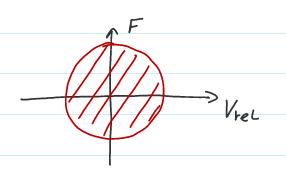
\includegraphics[width=0.4\linewidth]{figs/AktivniAktuator.png}
	\end{figure}

	\begin{figure}[h!]
		\centering
		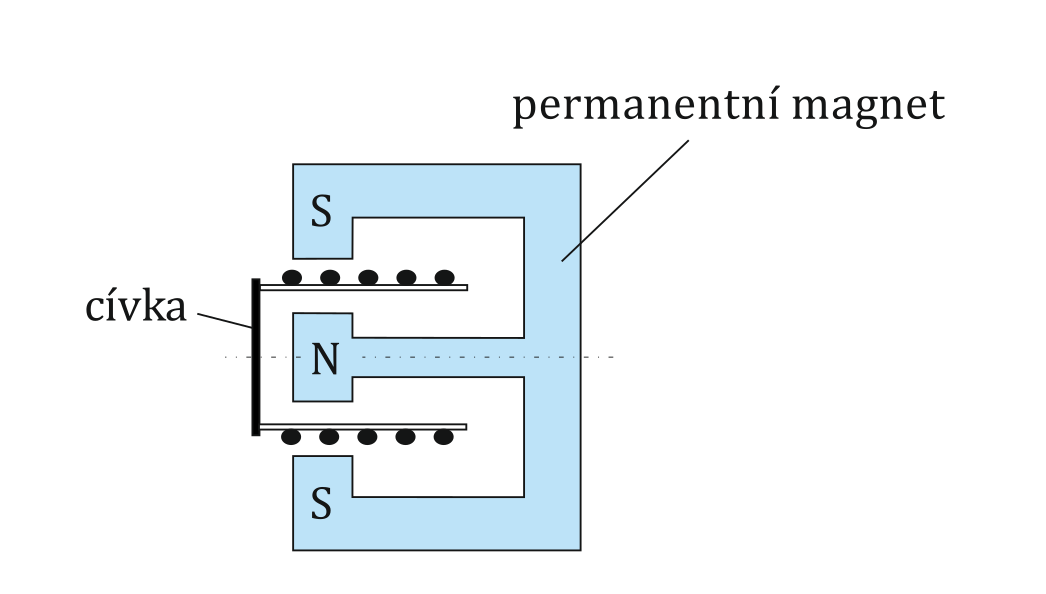
\includegraphics[width=0.3\linewidth]{figs/VoiceCoil.png}
		\caption{Voice coil}
	\end{figure}

	\subsection{Poloaktivní}
	Zdroje řízených tlumících sil (řízená disipace energie)
	\begin{itemize}
	\item tlumič s magnetoreologickou kapalinou
	\item tlumič se škrtícím ventilem
	\end{itemize}

	\begin{figure}[h!]
		\centering
		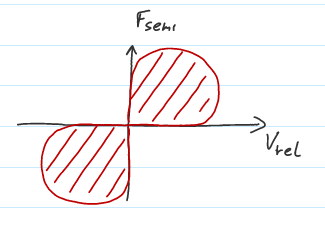
\includegraphics[width=0.4\linewidth]{figs/PoloAktivniAktuator.png}
	\end{figure}

	\section{Snižování vibrací (low-authority) versus řízení pohybu/polohy (high-authority). Princip, příklady}
	
	% Rozdělení na LAC a HAC vychází z předpokladu, že síly na řízeni pohybu jsou řádově vyšší než síly potřebné ke snížení vibrací. 
	\emph{``The control forces that act on a structure can be divided into tracking forces and damping forces. The tracking forces move the structure to follow a target and the damping forces act on the structure to suppress vibrations. Typically, the tracking forces are significantly larger than the damping forces. For this reason a structural controller can be divided into low- and high-authority controllers. The low-authority controller is the one that uses a limited input (torque, force) to control the vibrations of a system.''}

	\emph{`` the control system action on a flexible structure can be separated into two stages: stage one, when damping is added to a structure and vibrations are suppressed showing faster decay; and stage two, of “total” system motion where the damping is little affected.''}
	
	\subsection*{LAC}
	\begin{itemize}
		\item často využívá kolokace aktuátoru a senzoru, pro zvýšení robustnosti a decentralizované přístupy k řízení.
		\item Positive Position Feedback, Integral Force Feedback
	\end{itemize}

	\subsection*{HAC}
	\begin{itemize}
		\item Rekonstrukce stavů pomocí stavového pozorovatele
		\item Computed Torques, LQG (LQR + Kalman filtr)
	\end{itemize}

	\section{Aktivní absorbce kmitů soustav, příklad návrhu řízení}
	
	Využívá se antirezonance tzn. kmitání soustavy, při které je nulá výchlyka v místě buzení, zatímco kmitá jiná část soustavy. Pro tento účel se montují na mechanismy ``hltiče'' vibrací v podobě hmoty spojené se zbytkem soustavy pomocí aktivních prvků.

	Výsledkem připojení hltiče je systém ve tvaru
	\begin{align}
		\bm{\dot{x}} &= \bm{A}\bm{x} + \bm{B}\bm{u} + \bm{B}_\text{akt} \bm{u}_\text{akt} \\
		\bm{y} &= \bm{C}\bm{x}
	\end{align}
	Pokud máme přístup ke stavu systému, můžeme zavést lineární zpětnou vazbu
	\begin{equation}
		\bm{u}_\text{akt} = -\bm{K}\bm{x}
	\end{equation}
	s důsledkem na stavový popis
	\begin{equation}
		\bm{\dot{x}} = \underbrace{(\bm{A}-\bm{B}_h\bm{K})}_{A_\text{akt}}\bm{x} + \bm{B}\bm{u}
	\end{equation}
	Převodem do frekvenční oblasti získáme systém
	\begin{equation}
	\bm{y}(s) = \bm{H}(s)\bm{u}
	\;,\quad 
	\bm{H}(s) = \bm{C}(s\bm{I}-\bm{A}_\text{akt})^{-1}\bm{B}
	\end{equation}
	kde nuly přenosu $\bm{H}(s)$ můžeme manipulovat volbou $\bm{K}$.

	\section{Mechatronická tuhost. Princip, model, příklad návrhu řízení.}

	Koncept založený na použití pomocné sekundární struktury k navýšení dynamické tuhosti primární struktury a to jejich spojením pomocí aktivního prvku. Podmínka říditelnosti říká, že vlastní frekvence primární a sekundární struktury se musí lišit.

	\pagebreak
	\section{Aktivní tlumení vibrací pomocí kolokovaných aktuátorů a senzorů. Příklad s použitím planárních piezo-aktuátorů.}

	% \emph{``Collocated controllers have their sensors collocated with actuators. They are a special case of the dissipative controllers, which are designed based on the passivity principle.''}

	% \emph{``As a corollary, consider a system with the state-space representation $(\bm{A}, \bm{B}, \bm{C})$, which has collocated sensors and actuators, that is, $\bm{C}=\bm{B}^{T}$. In this case, a closedloop system with the proportional feedback gain
	% $$
	% \bm{u}=-\bm{K}\bm{y}
	% $$
	% is stable, for $\bm{K}=\operatorname{diag}\left(k_i\right), i=1, \ldots, r$ and $k_i>0$.''}

	% Asymptotická stabilita disipativního systému $(\bm{A}, \bm{B}, \bm{C})$, kde počet vstupů se rovná počtu výstupů, je zaručena při zpětnovazební regulaci ve tvaru
	% \begin{equation}
	% 	\bm{u}=-\bm{K}\bm{y}
	% \end{equation}
	% pokud matice $\bm{K}$ je pozitivně definitní.

	Systém ve tvaru $(\bm{A}, \bm{B}, \bm{C})$, který má stejný počet vstupů a výstupů nazveme striktně dispativní pokud existuje pozitivně definitní matice $\bm{P}$ a matice $\bm{Q}$ takové, že
	\begin{align}
		\bm{A}^T\bm{P} + \bm{P}\bm{A} &= \bm{Q}^T\bm{Q} \\
		\bm{B}^T\bm{P} &= \bm{C}
	\end{align}
	a $\bm{Q}^T\bm{Q}$ je pozitivně semi-definitní. Obecná podmínka asymptotické stability disipativního systému je, že ve zpětné vazbě
	\begin{equation}
		\bm{u}=-\bm{K}\bm{y}
	\end{equation}
	je matice $\bm{K}$ je pozitivně definitní.

	Systém s kolokovanými senzory a aktuátory je speciální případ disipativního systému kde $\bm{C}=\bm{B}^{T}$. Matice $\bm{K}$ je například pozitivně definitní pokud $\bm{K}=\operatorname{diag}\left(k_i\right), k_i>0$ kdy se jedná u kolokovaného systému o PPF.

	% osobně si myslím, že by stačilo CB je diag a poz def

	\pagebreak
	\section{Aktivní vibroizolace soustav, integrální silová zpětná vazba, příklad návrhu řízení.}

	Nahradíme piezostackem s tuhostí $k$, nastavitelnou volnou délkou $l_0(u) = l_{00} + qu$ a pozitivní, integrální, silovou zpětnou vazbou $u = p \int F\,dt$, kde $p$ je volitelný parametr.

	Pohybová rovnice systému bude nabývat tvar
	\begin{equation}
		m\ddot{y} = - \underbrace{k ( y-z_0(t)-qu)}_{F}
	\end{equation}
	Dosazením z pohybové rovnice můžeme určit tvar akčního zásahu
	\begin{align}
		u = p \int F\,dt = p \int -m\ddot{y} = -pm\dot{y} + C
	\end{align}

	Dosazením tvaru akčního zásahu zpět do pohybové rovnice získáme pohybovou rovnici tlumeného systému
	\begin{equation}
		m\ddot{y} = -k (y-z_0(t)) - \underbrace{kmpq}_{b_{\text{sky}}}\dot{y} - kqC
	\end{equation}
	kde hodnotu $b_{\text{sky}}$ můžeme ladit volbou parametru $p$

	\section{Říditelnost a pozorovatelnost, Gramián říditelnosti a pozorovatelnosti}

	Uvažujme lin. systém ve tvaru
	\begin{align*}
		\bm{\dot{x}} &= \bm{A}\bm{x} + \bm{B}\bm{u} \\
		\bm{y} &= \bm{C}\bm{x} + \bm{D}\bm{u}
	\end{align*}

	\subsection*{Říditelnost}
	Systém je říditelný pokud jej lze z libovolného stavu $\bm{x} \in \mathbb{R}^n$ dostat do stavu nulového $\bm{x} = \bm{0}$ působením vstupů $\bm{u}$.

	\subsubsection*{Matice říditelnosti}
	\begin{equation}
		\bm{\mathcal{C}}
		=
		\begin{bmatrix}
			\bm{B} & \bm{A} \bm{B} & \bm{A}^{2} \bm{B} & \dots & \bm{A}^{n-1} \bm{B}
		\end{bmatrix}
	\end{equation}
	Pokud $\bm{\mathcal{C}}$ je plné hodnosti, systém je říditelný.

	\subsubsection*{Gramián říditelnosti}
	\begin{equation}
		\bm{W}_{c}
		=
		\int_{0}^{\infty} e^{\bm{A} \tau} \bm{B} \bm{B}^T e^{\bm{A}^T \tau} d \tau
	\end{equation}
	Vlastní vektory $\bm{W}_c$ patřící k největším vlastním číslům jsou nejlépe říditelné směry ve stavovém prostoru. Podmíněností $\bm{W}_c$ můžeme hodnotit celkovou říditelnost systému (ve všech směrech stavového prostoru).

	\subsection*{Pozorovatelnost}
	Systém je pozorovatelný pokud na konečném časovém intervalu lze ze změřeného průběhu vstupů $\bm{u}$ a výstupů $\bm{y}$ určit stav systému na počátku invervalu $\bm{x}_0 \in \mathbb{R}^n$.
	
	\subsubsection*{Matice pozorovatelnosti}
	\begin{equation}
		\bm{\mathcal{O}}
		=
		\begin{bmatrix}
			\bm{C} \\
			\bm{C} \bm{A} \\
			\bm{C} \bm{A}^{2} \\
			\vdots \\
			\bm{C} \bm{A}^{n-1}
		\end{bmatrix}
	\end{equation}
	Pokud $\bm{\mathcal{O}}$ je plné hodnosti, systém je pozorovatelný.

	\subsubsection*{Gramián pozorovatelnosti}
	\begin{equation}
		\bm{W}_{o}
		=
		\int_{0}^{\infty} e^{\bm{A} \tau} \bm{C} \bm{C}^T e^{\bm{A}^T \tau} d \tau
	\end{equation}
	Vlastní vektory $\bm{W}_o$ patřící k největším vlastním číslům jsou nejlépe pozorovatelné směry ve stavovém prostoru. Podmíněností $\bm{W}_o$ můžeme hodnotit celkovou pozorovatelnost systému (ve všech směrech stavového prostoru).

	\section{Computed Torques}
	\begin{equation}
	\bm{M}(\bm{q}) + \bm{N}(\bm{q},\bm{\dot{q}}) = \bm{\tau}
	\end{equation}

	\begin{align}
		\bm{e} &= \bm{q}_{d}-\bm{q} \\
		\bm{\dot{e}} &= \bm{\dot{q}}_{d}-\bm{\dot{q}} \\
		\bm{\ddot{e}}
		&=
		\bm{\ddot{q}}_{d}-\bm{\ddot{q}}
		=
		\bm{\ddot{q}}_{d}-\bm{M}(\bm{q})^{-1} \bm{\tau}+\bm{M}(\bm{q})^{-1} \bm{N}(\bm{q},\bm{\dot{q}})
	\end{align}

	\begin{equation}
		\frac{d}{d t}
		\begin{bmatrix}
			\bm{e} \\
			\bm{\dot{e}}
		\end{bmatrix}
		=
		\begin{bmatrix}
			\bm{0} & \bm{I} \\
			\bm{0} & \bm{0}
		\end{bmatrix}
		\begin{bmatrix}
			\bm{e} \\
			\bm{\dot{e}}
		\end{bmatrix}
		+	
		\begin{bmatrix}
			\bm{0} \\
			\bm{I}
		\end{bmatrix}
		\bm{u}
	\end{equation}

	\begin{align}
		\bm{\ddot{e}} &= \bm{u} \\
		\bm{u} &= -k_p \bm{e} - k_d \bm{\dot{e}} - k_i \bm{\varepsilon}
		\;,\quad 
		\bm{\dot{\varepsilon}} = \bm{e} 
	\end{align}

	\begin{equation}
		\bm{\tau} = \bm{M}(\bm{q}) ( \bm{\ddot{q}}_d + k_p \bm{e} + k_d \bm{\dot{e}} + k_i \bm{\varepsilon} ) + \bm{N}(\bm{q},\bm{\dot{q}})
	\end{equation}

	\section{Použití optimalizačních metod pro syntézu řízení. Aktivní a poloaktivní aktuátory, lineární a nelineární soustavy (ilustrace na příkladu nelineární soustavy).}


\end{document}